 %  A simple AAU report template.
%  2015-05-08 v. 1.2.0
%  Copyright 2010-2015 by Jesper Kjær Nielsen <jkn@es.aau.dk>
%
%  This is free software: you can redistribute it and/or modify
%  it under the terms of the GNU General Public License as published by
%  the Free Software Foundation, either version 3 of the License, or
%  (at your option) any later version.
%
%  This is distributed in the hope that it will be useful,
%  but WITHOUT ANY WARRANTY; without even the implied warranty of
%  MERCHANTABILITY or FITNESS FOR A PARTICULAR PURPOSE.  See the
%  GNU General Public License for more details.
%
%  You can find the GNU General Public License at <http://www.gnu.org/licenses/>.
%
%  A simple AAU report template.
%  2015-05-08 v. 1.2.0
%  Copyright 2010-2015 by Jesper Kjær Nielsen <jkn@es.aau.dk>
%
%  This is free software: you can redistribute it and/or modify
%  it under the terms of the GNU General Public License as published by
%  the Free Software Foundation, either version 3 of the License, or
%  (at your option) any later version.
%
%  This is distributed in the hope that it will be useful,
%  but WITHOUT ANY WARRANTY; without even the implied warranty of
%  MERCHANTABILITY or FITNESS FOR A PARTICULAR PURPOSE.  See the
%  GNU General Public License for more details.
%
%  You can find the GNU General Public License at <http://www.gnu.org/licenses/>.
%
\documentclass[11pt,a4paper,openany]{report}
%%%%%%%%%%%%%%%%%%%%%%%%%%%%%%%%%%%%%%%%%%%%%%%%
% Language, Encoding and Fonts
% http://en.wikibooks.org/wiki/LaTeX/Internationalization
%%%%%%%%%%%%%%%%%%%%%%%%%%%%%%%%%%%%%%%%%%%%%%%%
% Select encoding of your inputs. Depends on
% your operating system and its default input
% encoding. Typically, you should use
%   Linux  : utf8 (most modern Linux distributions)
%            latin1 
%   Windows: ansinew
%            latin1 (works in most cases)
%   Mac    : applemac
% Notice that you can manually change the input
% encoding of your files by selecting "save as"
% an select the desired input encoding. 
\usepackage[utf8]{inputenc}
% Make latex understand and use the typographic
% rules of the language used in the document.
\usepackage[italian]{babel}
% Use the palatino font
\usepackage[sc]{mathpazo}
\linespread{1.05}         % Palatino needs more leading (space between lines)
% Choose the font encoding
\usepackage[T1]{fontenc}
%%%%%%%%%%%%%%%%%%%%%%%%%%%%%%%%%%%%%%%%%%%%%%%%
% Graphics and Tables
% http://en.wikibooks.org/wiki/LaTeX/Importing_Graphics
% http://en.wikibooks.org/wiki/LaTeX/Tables
% http://en.wikibooks.org/wiki/LaTeX/Colors
%%%%%%%%%%%%%%%%%%%%%%%%%%%%%%%%%%%%%%%%%%%%%%%%
% load a colour package
\usepackage[dvipsnames]{xcolor}
\definecolor{aaublue}{RGB}{33,26,82}% dark blue
% The standard graphics inclusion package
\usepackage{graphicx}
% Set up how figure and table captions are displayed
\usepackage{caption}
\captionsetup{%
  font=footnotesize,% set font size to footnotesize
  labelfont=bf % bold label (e.g., Figure 3.2) font
}
% Make the standard latex tables look so much better
\usepackage{array,booktabs}
% Enable the use of frames around, e.g., theorems
% The framed package is used in the example environment
\usepackage{framed}

%%%%%%%%%%%%%%%%%%%%%%%%%%%%%%%%%%%%%%%%%%%%%%%%
% Mathematics
% http://en.wikibooks.org/wiki/LaTeX/Mathematics
%%%%%%%%%%%%%%%%%%%%%%%%%%%%%%%%%%%%%%%%%%%%%%%%
% Defines new environments such as equation,
% align and split 
\usepackage{amsmath}
% Adds new math symbols
\usepackage{amssymb}
% Use theorems in your document
% The ntheorem package is also used for the example environment
% When using thmmarks, amsmath must be an option as well. Otherwise \eqref doesn't work anymore.
\usepackage[framed,amsmath,thmmarks]{ntheorem}

%%%%%%%%%%%%%%%%%%%%%%%%%%%%%%%%%%%%%%%%%%%%%%%%
% Page Layout
% http://en.wikibooks.org/wiki/LaTeX/Page_Layout
%%%%%%%%%%%%%%%%%%%%%%%%%%%%%%%%%%%%%%%%%%%%%%%%
% Change margins, papersize, etc of the document
\usepackage[a4paper, total={6in, 8in}]{geometry}
% Modify how \chapter, \section, etc. look
% The titlesec package is very configureable
\usepackage{titlesec}
\titleformat{\chapter}[display]{\normalfont\huge\bfseries}{\chaptertitlename\ \thechapter}{20pt}{\Huge}
\titleformat*{\section}{\normalfont\Large\bfseries}
\titleformat*{\subsection}{\normalfont\large\bfseries}
\titleformat*{\subsubsection}{\normalfont\normalsize\bfseries}
%\titleformat*{\paragraph}{\normalfont\normalsize\bfseries}
%\titleformat*{\subparagraph}{\normalfont\normalsize\bfseries}
% Change the headers and footers
\usepackage{fancyhdr}
\pagestyle{fancy}
\fancyhf{}
\fancyhead[L]{\rightmark}
\fancyfoot[C]{\thepage}
\renewcommand{\headrulewidth}{0pt}

% Do not stretch the content of a page. Instead,
% insert white space at the bottom of the page
\raggedbottom
% Enable arithmetics with length. Useful when
% typesetting the layout.
\usepackage{calc}


%%%%%%%%%%%%%%%%%%%%%%%%%%%%%%%%%%%%%%%%%%%%%%%%
% Bibliography
% http://en.wikibooks.org/wiki/LaTeX/Bibliography_Management
%%%%%%%%%%%%%%%%%%%%%%%%%%%%%%%%%%%%%%%%%%%%%%%%
\usepackage[backend=bibtex,
  bibencoding=utf8
  ]{biblatex}
\addbibresource{bib/mybib}

%%%%%%%%%%%%%%%%%%%%%%%%%%%%%%%%%%%%%%%%%%%%%%%%
% Misc
%%%%%%%%%%%%%%%%%%%%%%%%%%%%%%%%%%%%%%%%%%%%%%%%
% Add bibliography and index to the table of
% contents
\usepackage[nottoc]{tocbibind}
% Add the command \pageref{LastPage} which refers to the
% page number of the last page
\usepackage{lastpage}

\usepackage{float}
% Add todo notes in the margin of the document
\usepackage[
%  disable, %turn off todonotes
  colorinlistoftodos, %enable a coloured square in the list of todos
  textwidth=\marginparwidth, %set the width of the todonotes
  textsize=scriptsize, %size of the text in the todonotes
  ]{todonotes}

%%%%%%%%%%%%%%%%%%%%%%%%%%%%%%%%%%%%%%%%%%%%%%%%
% Hyperlinks
% http://en.wikibooks.org/wiki/LaTeX/Hyperlinks
%%%%%%%%%%%%%%%%%%%%%%%%%%%%%%%%%%%%%%%%%%%%%%%%
% Enable hyperlinks and insert info into the pdf
% file. Hypperref should be loaded as one of the 
% last packages
\usepackage[hidelinks]{hyperref}
\hypersetup{%
	pdfpagelabels=true,%
	plainpages=false,%
	pdfauthor={Author(s)},%
	pdftitle={Title},%
	pdfsubject={Subject},%
	bookmarksnumbered=true,%
	colorlinks=false,%
	citecolor=black,%
	filecolor=black,%
	linkcolor=black,% you should probably change this to black before printing
	urlcolor=black,%
	pdfstartview=FitH%
}

\newcommand{\quotes}[1]{``#1''}
\usepackage{catchfile}
\usepackage{listings}
\usepackage{adjustbox}
\usepackage{makecell}


\lstset{
	float,
	basicstyle=\ttfamily,
	frame=single
}

\usepackage{multirow}
\usepackage{makecell}

% package inclusion and set up of the document
% see, e.g., http://en.wikibooks.org/wiki/LaTeX/Formatting#Hyphenation
% for more information on word hyphenation
\hyphenation{ex-am-ple hy-phen-a-tion short}
\hyphenation{long la-tex}% 
%  A simple AAU report template.
%  2015-05-08 v. 1.2.0
%  Copyright 2010-2015 by Jesper Kjær Nielsen <jkn@es.aau.dk>
%
%  This is free software: you can redistribute it and/or modify
%  it under the terms of the GNU General Public License as published by
%  the Free Software Foundation, either version 3 of the License, or
%  (at your option) any later version.
%
%  This is distributed in the hope that it will be useful,
%  but WITHOUT ANY WARRANTY; without even the implied warranty of
%  MERCHANTABILITY or FITNESS FOR A PARTICULAR PURPOSE.  See the
%  GNU General Public License for more details.
%
%  You can find the GNU General Public License at <http://www.gnu.org/licenses/>.
%
%
%
% see, e.g., http://en.wikibooks.org/wiki/LaTeX/Customizing_LaTeX#New_commands
% for more information on how to create macros

%%%%%%%%%%%%%%%%%%%%%%%%%%%%%%%%%%%%%%%%%%%%%%%%
% Macros for the titlepage
%%%%%%%%%%%%%%%%%%%%%%%%%%%%%%%%%%%%%%%%%%%%%%%%
%Creates the aau titlepage
\newcommand{\aautitlepage}[3]{%
  {
    %set up various length
    \ifx\titlepageleftcolumnwidth\undefined
      \newlength{\titlepageleftcolumnwidth}
      \newlength{\titlepagerightcolumnwidth}
    \fi
    \setlength{\titlepageleftcolumnwidth}{0.5\textwidth-\tabcolsep}
    \setlength{\titlepagerightcolumnwidth}{\textwidth-2\tabcolsep-\titlepageleftcolumnwidth}
    %create title page
    \thispagestyle{empty}
    \noindent%
    \begin{tabular}{@{}ll@{}}
      \parbox{\titlepageleftcolumnwidth}{
        \iflanguage{danish}{%
          \includegraphics[width=\titlepageleftcolumnwidth]{figures/aau_logo_da}
        }{%
          \includegraphics[width=\titlepageleftcolumnwidth]{figures/aau_logo_en}
        }
      } &
      \parbox{\titlepagerightcolumnwidth}{\raggedleft\sf\small
        #2
      }\bigskip\\
       #1 &
      \parbox[t]{\titlepagerightcolumnwidth}{%
      \textbf{Abstract:}\bigskip\par
        \fbox{\parbox{\titlepagerightcolumnwidth-2\fboxsep-2\fboxrule}{%
          #3
        }}
      }\\
    \end{tabular}
    \vfill
    \iflanguage{danish}{%
      \noindent{\footnotesize\emph{Rapportens indhold er frit tilgængeligt, men offentliggørelse (med kildeangivelse) må kun ske efter aftale med forfatterne.}}
    }{%
      \noindent{\footnotesize\emph{The content of this report is freely available, but publication (with reference) may only be pursued due to agreement with the author.}}
    }
    \clearpage
  }
}

%Create english project info
\newcommand{\englishprojectinfo}[8]{%
  \parbox[t]{\titlepageleftcolumnwidth}{
    \textbf{Title:}\\ #1\bigskip\par
    \textbf{Theme:}\\ #2\bigskip\par
    \textbf{Project Period:}\\ #3\bigskip\par
    \textbf{Project Group:}\\ #4\bigskip\par
    \textbf{Participant(s):}\\ #5\bigskip\par
    \textbf{Supervisor(s):}\\ #6\bigskip\par
    \textbf{Copies:} #7\bigskip\par
    \textbf{Page Numbers:} \pageref{LastPage}\bigskip\par
    \textbf{Date of Completion:}\\ #8
  }
}

%Create danish project info
\newcommand{\danishprojectinfo}[8]{%
  \parbox[t]{\titlepageleftcolumnwidth}{
    \textbf{Titel:}\\ #1\bigskip\par
    \textbf{Tema:}\\ #2\bigskip\par
    \textbf{Projektperiode:}\\ #3\bigskip\par
    \textbf{Projektgruppe:}\\ #4\bigskip\par
    \textbf{Deltager(e):}\\ #5\bigskip\par
    \textbf{Vejleder(e):}\\ #6\bigskip\par
    \textbf{Oplagstal:} #7\bigskip\par
    \textbf{Sidetal:} \pageref{LastPage}\bigskip\par
    \textbf{Afleveringsdato:}\\ #8
  }
}

%%%%%%%%%%%%%%%%%%%%%%%%%%%%%%%%%%%%%%%%%%%%%%%%
% An example environment
%%%%%%%%%%%%%%%%%%%%%%%%%%%%%%%%%%%%%%%%%%%%%%%%
\theoremheaderfont{\normalfont\bfseries}
\theorembodyfont{\normalfont}
\theoremstyle{break}
\def\theoremframecommand{{\color{gray!50}\vrule width 5pt \hspace{5pt}}}
\newshadedtheorem{exa}{Example}[chapter]
\newenvironment{example}[1]{%
		\begin{exa}[#1]
}{%
		\end{exa}
}% my new macros

\begin{document}
%frontmatter
\pagestyle{empty} %disable headers and footers
\pagenumbering{roman} %use roman page numbering in the frontmatter
%  A simple AAU report template.
%  2015-05-08 v. 1.2.0
%  Copyright 2010-2015 by Jesper Kjær Nielsen <jkn@es.aau.dk>
%
%  This is free software: you can redistribute it and/or modify
%  it under the terms of the GNU General Public License as published by
%  the Free Software Foundation, either version 3 of the License, or
%  (at your option) any later version.
%
%  This is distributed in the hope that it will be useful,
%  but WITHOUT ANY WARRANTY; without even the implied warranty of
%  MERCHANTABILITY or FITNESS FOR A PARTICULAR PURPOSE.  See the
%  GNU General Public License for more details.
%
%  You can find the GNU General Public License at <http://www.gnu.org/licenses/>.
%
\pdfbookmark[0]{Front page}{label:frontpage}%
\begin{titlepage}
  \addtolength{\hoffset}{0.5\evensidemargin-0.5\oddsidemargin} %set equal margins on the frontpage - remove this line if you want default margins
  \noindent%
  \begin{tabular}{@{}p{\textwidth}@{}}
    \toprule[2pt]
    \midrule
    \vspace{0.2cm}
    \begin{center}
    \Huge{\textbf{
      Progetto Modelli Probabilistici\\per le Decisioni% insert your title here
    }}
    \end{center}
    \begin{center}
      \Large{
        - Relazione finale -% insert your subtitle here
      }
    \end{center}
    \vspace{0.2cm}\\
    \midrule
    \toprule[2pt]
  \end{tabular}
  \vspace{4 cm}
  \begin{center}
    \vspace{0.2cm}
    {\Large
     	Lorenzo Mammana 807391\\
		Eric Nisoli 807147
     	%Insert your group name or real names here
    }
  \end{center}
  \vfill
  \begin{center}
  Università degli Studi di Milano-Bicocca\\
  2018/2019
  \end{center}
\end{titlepage}
\clearpage
\pdfbookmark[0]{Contents}{label:contents}
\pagestyle{fancy} %enable headers and footers again
\tableofcontents
\cleardoublepage
%mainmatter
\pagenumbering{arabic} %use arabic page numbering in the mainmatter
\chapter{Introduzione}\label{ch:intro}

Almeno una volta nella vita, durante la fase di studi, un musicista dovrebbe avere eseguito l'armonizzazione di un corale. Questo compito consiste nel, data una certa melodia, creare tre melodie sottostanti che suonate assieme siano piacevoli all'ascolto. \\
Ciò viene richiesto ai musicisti in quanto è abbastanza aperto per valutare le capacità dello studente, ma allo stesso tempo data la presenza di strutture piuttosto rigorose, è vincolato abbastanza da non richiedere una composizione libera. \\
L'obiettivo del progetto è quello di verificare se questo compito è fattibile tramite algoritmi di apprendimento automatico e se i risultati prodotti siano o meno confondibili con risultati reali.\\
Numerose tecniche sono state presentate in letterature per svolgere questo compito, alcuni approcci basati su reti neurali, altri basati su algoritmi genetici, ma la maggior parte basati su Hidden Markov Models (HMM). \\
Il nostro lavoro è completamente basato sul paper [citare paper] che descrive, oltre ad un HMM in grado di eseguire il task di armonizzazione, anche un secondo HMM in grado di eseguire il compito di ornamentazione, ovvero l'aggiunta di note ininfluenti per la melodia, ma in grado di aggiungere quella fantasia compositiva in più che ci si aspetta da un musicista reale.

\chapter{Operazioni preliminari}\label{ch:th-music}

\section{Disclaimer}
Gli autori non sono musicisti, ne hanno mai studiato musica! \\
La nostra conoscenza in merito è stata costruita nel periodo del progetto e come tale potranno esserci inesattezze nella terminologia utilizzata.

\section{Dataset}
Il dataset utilizzato è costituito da 382 corali composti da Johann Sebastian Bach in formato testuale come mostrato nel Listing \ref{music-notation}.
Dall'header estraiamo alcune informazioni importanti come:
\begin{itemize}
\item Tonart: rappresenta la tonalità con cui è composto il corale (dur = Maggiore, moll = Minore)
\item Takt: rappresenta la time signature del corale
\item Tempo: rappresenta la velocità del corale
\end{itemize}
\lstinputlisting[label={music-notation},
	caption={Struttura musicale del corale 10},
	captionpos=b,
	language={}]
	{listings/music-notation.txt}
\noindent
In particolare la notazione utilizzata per descrivere la tonalità è quella utilizzata principalmente nelle zone di influenza germanica, la conversione ad un sistema a noi più familiare è immediata.
\begin{table}[H]
\centering
\begin{tabular}{|l|l|l|l|l|l|l|}
\hline
A  & H  & C  & D  & E   & F  & G  \\ \hline
Do & Re & Mi & Fa & Sol & La & Si \\ \hline
\end{tabular}
\end{table}
\noindent
La composizione vera e propria si articola su diverse colonne:
\begin{itemize}
\item Il numero contenuto nella prima colonna rappresenta l'inizio di una frase (unità musicale che ha senso anche se suonata singolarmente)
\item Il numero contenuto nella seconda colonna rappresenta l'inizio di una nuova battuta
\item La terza colonna rappresenta la nota eseguita dal soprano
\item La quarta colonna rappresenta la nota eseguita dal contralto
\item La quinta colonna rappresenta la nota eseguita dal tenore
\item La sesta colonna rappresenta la nota eseguita dal basso
\item L'ultima colonna ci da un'indicazione riguardo la funzione armonica di una certa battuta.
\end{itemize}
\noindent
Il dataset viene inizialmente suddiviso in corali in tonalità maggiore e corali in tonalità minore in quanto la loro composizione è nettamente diversa.

\section{Preprocessing}
Il dataset così definito è ovviamente impossibile da utilizzare per addestrare un HMM, è necessario, per ogni file, costruire una coppia [stato nascosto-stato visibile] che sia in grado di rappresentarne la struttura musicale. \\
Questa operazione viene effettuata tramite lo script hmm-data.py, che legge i corali e costruisce l'input per il modello di Markov.
In particolare gli stati visibili rappresentano le note relative al soprano, mentre gli stati nascosti rappresentano le corde e la loro relativa funzione armonica. \\
Per ogni corale in ingresso viene prodotto un file $f$ con lo stesso nome contenente una sequenza $S_f(h, v)$ di coppie di indici come mostrato nel Listing \ref{data-out},
\lstinputlisting[label={data-out},
	caption={Esempio di file processato},
	captionpos=b,
	language={}]
	{listings/data-out.txt}
\noindent
a cui fanno riferimento rispettivamente gli stati nascosti e gli stati visibili contenuti nei file "SYMBOLS\_HIDDEN" e "SYMBOLS\_VISIBLE".
Come vediamo nel Listing \ref{hid-vis-a} (a) uno stato nascosto è nella forma a:b:c:0/Y, dove a rappresenta il numero di semitoni in più del soprano rispetto al basso, in maniera equivalente b e c rappresentano il numero di semitoni in più di contralto e tenore rispetto al basso. \\
Nel Listing \ref{hid-vis-b} (b) vediamo invece come gli stati visibili siano semplicemente le note della melodia del soprano.

\begin{center}
\begin{minipage}[t]{.45\textwidth}
	\lstinputlisting[label={hid-vis-a},
		title={(a)},
		language={}]
		{listings/hid-vis-a.txt}
\end{minipage}
\hspace{.5cm}
\begin{minipage}[t]{.45\textwidth}
	\lstinputlisting[label={hid-vis-b},
		title={(b)},
		language={}]
		{listings/hid-vis-b.txt}
\end{minipage}
\captionof{lstlisting}{(a) Inizio del file SYMBOLS\_HIDDEN (b) Inizio del file SYMBOLS\_VISIBLE}
\end{center}
\chapter{Chords HMM}\label{ch:hmm-chords}
Identifichiamo la sequenza di note della melodia con Y e l'armonizzazione sottostante con C, in particolare $y_t$ rappresenta la nota della melodia al tempo t e $c_t$ rappresenta lo stato armonico al tempo t. \\
E' stato utilizzato un modello di Markov con assunzioni del primo ordine, ovvero tale per cui vale:
\begin{equation}
P(c_t|c_{t-1},...,c_0) = P(c_t|c_{t-1})
\end{equation}
\begin{equation}
P(y_t|c_t,...,c_0,y_{t-1},...,y_0) = P(y_t|c_t)
\end{equation}
In particolare vengono costruiti due modelli di Markov, uno relativo ai corali in tonalità maggiore ed uno relativo ai corali in tonalità minore.
Il dataset iniziale è stato così suddiviso:
\begin{itemize}
\item 121 file di training (tonalità maggiore)
\item 81 file di test (tonalità maggiore)
\item 108 file di training (tonalità minore)
\item 72 file di test (tonalità minore)
\end{itemize}
\section{Training}
Il modello di Markov è stato costruito utilizzando la libreria Python "hmmlearn". \\
Avendo a disposizione sia gli stati visibili che gli stati nascosti non è stato necessario apprendere i parametri del modello tramite Expected Maximization, ma sono state invece costruite, utilizzando i dati, sia la matrice di transizione che la matrice di emissione.\\
In particolare per gestire il grande numero di zero all'interno di queste matrici si è proceduto applicando uno smoothing additivo sommando 0.01 ad ogni elemento delle matrici prima di normalizzarle per renderle stocastiche.
Anche la distribuzione iniziale di probabilità è stata calcolata utilizzando i dati, andando a dare una probabilità maggiore agli stati più frequenti all'inizio dei corali. \\
Il modello relativo alla tonalità maggiore (chords-dur) contiene 2815 stati nascosti e 55 stati visibili, mentre il modello relativo alla tonalità minore (chords-moll) contiene 2593 stati nascosti e 52 stati visibili.
\section{Testing}
Per ogni file di test viene generata, data la relativa sequenza di stati visibili, la sequenza più probabile di stati nascosti utilizzando l'algoritmo di Viterbi.
In tabella viene mostrato quanto gli stati nascosti prodotti siano equivalenti a quelli reali. \\
INSERIRE TABELLA RISULTATI
Come ci si aspetta i risultati sono abbastanza diversi in quanto il modello non ha alcuna informazione relativa ad esempio al periodo in cui è stato composto un determinato corale, oppure per quale occasione. Senza l'ausilio di ulteriori dati esterni sarebbe impossibile ricostruire perfettamente i corali originali.
\begin{figure}[H]
	\centering
	\caption{A sx l'originale, a dx l'armonizzazione più probabile del nostro modello}
	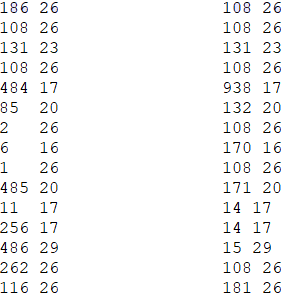
\includegraphics{figures/viterbi.png}
	\label{viterbi}
\end{figure}
\noindent
Interpretare i risultati non è semplice, la figura \ref{viterbi} non è per nulla esplicativa, se ragionassimo in termini di accuratezza sembrerebbe che il nostro modello sia assolutamente pessimo, ma l'obiettivo non è quello di costruire risultati identici all'originale, ma armonizzazioni musicalmente accettabili e orecchiabili. \\
Presentare i risultati sotto forma di spartito musicale può favorirne la comprensione per chi è in grado di leggerli, ma non è abbastanza per chi non ha una approfondita conoscenza del dominio. Per questo motivo è necessario trasformare i risultati ottenuti in un formato musicale udibile.
\section{Sampling}
E' possibile anche generare sequenze di stati in accordo alla distribuzione di probabilità del modello. Consideriamo $\alpha_{t-1}(j)$, la probabilità di avere visto le prime $t - 1$ osservazioni di una sequenza ed essere finiti nello stato j, possiamo calcolare la probabilità di aver visto i primi $t - 1$ eventi, essere finiti in uno stato qualsiasi, e poi eseguire una transizione verso uno stato k:
\begin{equation}
\begin{aligned}
P(y_0 = Y_{i0}, y_1 = Y_{i1}, ...,y_{t-1}=Y_{i_{t-1}},s_{t-1}=S_j, s_t=S_k) \\
	=\alpha_{t-1}(j)P(s_t=S_k|s_{t-1}=S_j)
\end{aligned}
\end{equation}
Possiamo usare questa equazione per calcolare $\rho_t(j|k)$ la probabilità di essere in uno stato $S_j$ al tempo $t-1$ data la sequenza di eventi osservati $Y_{i0}, Y_{i1},...,Y_{i{t-1}}$ e dato che saremo nello stato $S_k$ al tempo $t$:
\begin{equation}
\begin{aligned}
\rho_t(j|k)=P(s_{t-1}=S_j|y_0 = Y_{i0}, y_1 = Y_{i1}, ...,y_{t-1}=Y_{i_{t-1}}, s_t=S_k) \\
= \frac{\alpha_{t-1}(j)P(s_t=S_k|s_{t-1}=S_j)}{\sum_{l}P(s_t=S_k|s_{t-1}=S_l)}
\end{aligned}
\end{equation}
Per instanziare una sequenza di stati $s0=S_{v0},s1=S_{v1},...,s_T=s_{vT}$ viene inizialmente scelto lo stato finale utilizzando la distribuzione di probabilità del modello:
\begin{equation}
P(s_T=S_j|y_0=Y_{i0},y_1=Y_{i1},...,y_T=Y_{iT}) = \frac{\alpha_T(j)}{\sum_l\alpha_T(l)}
\end{equation}
Una volta scelto $v_T$ tale per cui lo stato finale risulti essere $s_t=S_{vt}$ possiamo usare le variabili $\rho_t(j|k)$ per muoverci all'indietro sulla sequenza:
\begin{equation}
P(s_T=S_j|y_0=Y_{i0},y_1=Y_{i1},...,y_T=Y_{iT}, s_{t+1}=S_{v_{t+1}}) = \rho_{t+1}(j|v_{t+1})
\end{equation}
\section{Ricostruzione dei risultati}
Mediante l'utilizzo dello script "hmm-output-expand.py" è possibile ricostruire, a partire dalle coppie [hidden-visible] costruite tramite Sampling o Viterbi, il file in notazione musicale.\\
In questo punto notiamo uno dei principali problemi del modello costruito, ovvero la mancanza di informazione temporale relativa agli stati visibili e nascosti. \\
Per ricostruire il file musicale è necessario rispettare le cadenze della musica originale e ciò rende molto complicato ad esempio generare nuova musica con il modello. Questo banalmente perchè la musica generata, per quanto orecchiabile, non avrà una struttura temporale sensata ed ogni nota avrà la stessa lunghezza, come tale la melodia prodotta risulterà molto "robotica" e poco reale.
\section{Generazione del file MIDI}
Il protocollo MIDI è uno standard per la composizione e riproduzione di file musicali. Tramite lo script "chorale2midi.py" è possibile convertire i file testuali generati nel passaggio precedente in formato MIDI in modo tale da poterli riprodurre. \\
\section{Armonizzazione di musica moderna}
Il modello di Markov proposto è teoricamente in grado di armonizzare una melodia qualsiasi, dato un file MIDI è possibile estrarre le note della melodia e utilizzarle come base per l'armonizzazione. Il task è però particolarmente complicato perchè la struttura dei file di input è molto rigida, in particolare:
\begin{itemize}
\item la durata delle note, nel file MIDI, deve necessariamente essere multiplo della durata di una nota semiminima (1/4)
\item in una battuta ci possono essere massimo quattro note
\item non c'è mai una pausa tra note nella stessa battuta
\end{itemize} 
Il primo motivo è facilmente gestibile andando ad arrotondare la durata delle note al multiplo più vicino, ciò altera leggermente la melodia, ma non abbastanza da rovinarla.\\
Il secondo è un problema legato principalmente a canzoni veloci o complesse che non sono gestibili dal modello. \\
L'ultimo problema è quello forse più complicato da gestire, in quanto richiede l'aggiunta di note fittizie all'interno del file che verranno poi trattate come delle pause.\\
In Python non sono presenti librerie in grado di gestire facilmente file MIDI in ingresso, per questo motivo la musica moderna è stata trascritta manualmente nei file testual e, per mancanza di tempo non è stato possibile effettuare automaticamente questo compito.
A questo si aggiunge il fatto che, molto spesso, i file MIDI non sono correttamente divisi per canali (idealmente uno strumento per canale) e ciò rende ancora più complicato il parsing automatico di questi file.\\
A puro scopo dimostrativo e ludico abbiamo provato ad armonizzare varie melodie moderne e non per vedere come suonerebbero se fossero state composte da Bach sotto forma di corale.
Nella maggior parte dei casi il suono è troppo cacofonico, principalmente quando la canzone è molto veloce o presenta una melodia con molte note per battuta.
\chapter{Ornamentation HMM}\label{ch:hmm-ornamentation}
Il primo modello di Markov aggiunge una sola nota per battuta per le linee melodiche di contralto, tenore e basso, questa è una semplificazione rispetto ai corali reali di Bach che possono invece presentare quattro note per battuta come accade per la linea melodica del soprano. Questo problema viene risolto addestrando un secondo modello di Markov nascosto in cui gli stati visibili rappresentano quanto le tre linee musicali crescono o decrescono tra una battuta ed un altra, mentre gli stati nascosti rappresentano di quanto dovrebbe essere alzato o abbassato uno degli ultimi tre quarti della battuta.
\begin{center}
	\begin{minipage}[h]{.45\textwidth}
		\lstinputlisting[label={hid-vis-orn-a},
		title={(a)},
		language={}]
		{listings/hid-vis-orn-a.txt}
	\end{minipage}
	\hspace{.5cm}
	\begin{minipage}[h]{.45\textwidth}
		\lstinputlisting[label={hid-vis-orn-b},
		title={(b)},
		language={}]
		{listings/hid-vis-orn-b.txt}
	\end{minipage}
	\captionof{lstlisting}{(a) Stati nascosti (b) Stati visibili}
	\label{hid-vis-orn}
\end{center}
\noindent
Ad esempio facendo riferimento all'ultima riga del Listato \ref{hid-vis-orn} vediamo che per una battuta in cui, nella battuta successiva, il contralto scende di 5 semitoni, il tenore scende di 2 semitoni e il basso scende di due semitoni andrà a generare le tre linee melodiche in cui la terza e la quarta nota sono rispettivamente abbassate di un semitono per contralto e tenore, ed alzate di due semitoni per il basso.
\section{Training}
Anche in questo caso prima del training viene effettuata una parte di preprocessing per ottenere gli stati visibili e nascosti, il training del modello viene eseguito esattamente come descritto nel capitolo precedente.
\section{Testing}
Anche in questo caso si opera nella stessa identica maniera descritta precedentemente, i risultati in termini di accuratezza vengono mostrati in tabella.
\section{Ricostruzione dei risultati}
Per ricostruire i risultati è stato necessario aggiungere uno script non presente nel repository originale in grado modificare il file musicale costruito dal modello di Markov precedente in accordo con la modifica di semitono delle linee melodiche.
\section{Generazione del file MIDI}
Una volta integrati i risultati dei due modelli è possibile costruire i file MIDI utilizzando lo stesso script relativo al modello precedente.
\section{Ornamentazione di musica moderna}
Non è invece possibile eseguire il task di ornamentazione della musica moderna, questo è dovuto al fatto che i file costruiti da noi contengono esclusivamente informazione relativa alla melodia del soprano e come tale non è possibile costruire gli stati visibili e nascosti richiesti dal modello per funzionare.
  
\chapter{Valutazione risultati}\label{ch:evaluation}
Non avendo conoscenze teoriche in merito alla musica la valutazione dei risultati è stata effettuata semplicemente andando a valutare la gradevolezza uditiva delle melodie composte dal modello.
In particolare sembra essere molto buona l'armonizzazione prodotta dal primo modello di Markov sui vari corali testati, questo soprattutto perchè il compito non è particolarmente complicato e molto spesso suonare più tasti del pianoforte assieme per lo stesso tempo produce suoni gradevoli.\\
I file prodotti tramite sampling basato su melodie note produce risultati simili a quelli di Viterbi, ma effettivamente peggiori all'ascolto.\\
Anche il test eseguito sulla musica moderna produce risultati interessanti, ovviamente la musica prodotta difficilmente potrebbe essere utilizzata realmente, ma soprattutto su parti lente e più vicine ai ritmi di un corale il modello armonizza bene e i risultati sono piuttosto gradevoli all'ascolto.\\
Il modello che esegue l'ornamentazione non ci convince invece particolarmente, molto spesso l'armonizzazione prodotta non è particolarmente gradevole, soprattutto se paragonata ai risultati prodotti dal modello precedente, in particolare abbiamo riscontrato una non riproducibilità dei risultati mostrati dall'autore dell'articolo. I suoi risultati sono eccezionali all'ascolto e sembrano veramente troppo perfetti per essere stati prodotti dal modello, è possibile che vi sia stata una manipolazione umana per rendere più interessante la proposta dell'articolo che, in ogni caso, presenta comunque un ottimo modello!
\chapter{Conclusioni}\label{ch:conclusions}
L'obiettivo ultimo del nostro lavoro era quello di rendere disponibile un modello di Markov per l'armonizzazione di corali funzionante e che non richiedesse di operare su file scritti in PERL, linguaggio molto popolare fino agli anni 2000, ma ormai in lento declino.\\
L'obiettivo è stato pienamente raggiunto, l'intero codice prodotto è scritto in Python ed è perfettamente utilizzabile come base per estendere il modello proposto con ulteriori idee e miglioramenti.\\
Il modello proposto da Allan si è rivelato funzionante, anche se in maniera inferiore a quanto mostrato dall'autore negli esempi che ha reso disponibili pubblicamente; il modello presenta però numerose lacune dovute soprattutto alla rigidità dei file di ingresso e alla scelta di non integrare alcuna informazione riguardante la durata delle note negli stati del modello. Questo causa l'impossibilità di generare automaticamente corali nello stile di Bach, da un certo punto di vista ciò è corretto, non è questo lo scopo che si è prefisso l'autore, da un altro punto di vista sarebbe stato interessante effettuare anche questo compito.\\
Il nostro maggior contributo oltre la traduzione è quello però di aver costruito script particolari in grado di prendere una linea melodica e costruirne l'armonizzazione, questo permette di verificare cosa succederebbe se Bach entrasse a far parte di un certo gruppo musicale. Questo ha fondamentalmente valenza ludica, il che non ne sminuisce comunque il valore, se consideriamo che il settore in questione è uno dei più importanti in ambito informatico.
\printbibliography[heading=bibintoc]
\label{bib:mybiblio}
\appendix
\end{document}